% !TEX program = pdflatex
% BT fork_wall no-aux agent: second experiment batch (8 figures).
\documentclass[11pt]{article}
\usepackage[margin=1in]{geometry}
\usepackage{graphicx}
\usepackage{amsmath}
\usepackage{caption}
\usepackage{float}
\usepackage[section]{placeins}
\usepackage{tikz}
\usetikzlibrary{arrows.meta, positioning, fit, backgrounds}
\captionsetup{font=small, labelfont=bf}
\newcommand{\code}[1]{\texttt{#1}}
\newcommand{\figdir}{figures/thesis_forkwall2}
\tikzset{
  blk/.style  = {draw, rounded corners, align=center, font=\small,
                 minimum height=2.5em, fill=blue!8, inner sep=4pt},
  rec/.style  = {draw, rounded corners, align=center, font=\small,
                 minimum height=2.5em, fill=green!10, inner sep=4pt},
  head/.style = {draw, rounded corners, align=center, font=\small,
                 minimum height=2.3em, fill=orange!14, inner sep=4pt},
  io/.style   = {draw, rounded corners, align=center, font=\small,
                 minimum height=2.5em, fill=gray!10, inner sep=4pt},
  fl/.style   = {-{Stealth[length=2.2mm]}, thick},
}

\title{\textbf{\code{fork\_wall} / no-aux agent: extended experiments}\\
\large training dynamics, skill use, generalisation, belief geometry,\\
probe-calibrated steering, and advance planning}
\author{}
\date{}

\begin{document}
\maketitle
\vspace{-2.5em}

\noindent All experiments use the reward-only (no auxiliary loss) PPO+GRU agent
from the \code{fork\_wall} chapter (GRU 128; success $0.99$). Evaluation maps
are held-out seeds; policies are sampled stochastically throughout.

% =====================================================================
\section*{The agent architecture}

\begin{figure}[H]
  \centering
  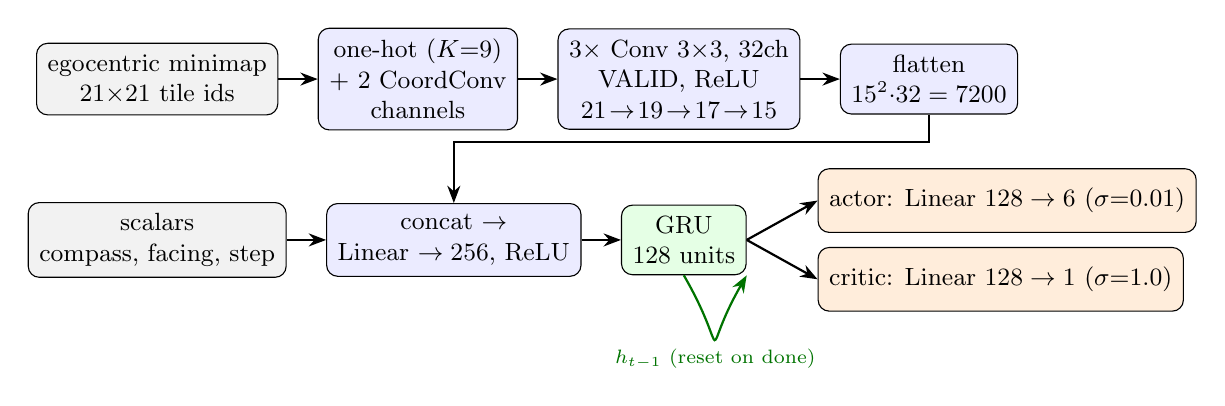
\begin{tikzpicture}[node distance=4mm and 5mm]
    % row 1: perception
    \node[io] (mm) {egocentric minimap\\ $21{\times}21$ tile ids};
    \node[blk, right=of mm] (oh) {one-hot ($K{=}9$)\\ $+$ 2 CoordConv\\ channels};
    \node[blk, right=of oh] (cnn) {$3\times$ Conv $3{\times}3$, 32ch\\ VALID, ReLU\\ $21\!\to\!19\!\to\!17\!\to\!15$};
    \node[blk, right=of cnn] (fl) {flatten\\ $15^2{\cdot}32 = 7200$};
    % row 2: memory + heads
    \node[io, below=11mm of mm] (sc) {scalars\\ compass, facing, step};
    \node[blk, right=of sc] (emb) {concat $\to$\\ Linear $\to 256$, ReLU};
    \node[rec, right=of emb] (gru) {GRU\\ 128 units};
    \node[head, right=9mm of gru, yshift=5mm] (act) {actor: Linear $128\to 6$ ($\sigma{=}0.01$)};
    \node[head, right=9mm of gru, yshift=-5mm] (cri) {critic: Linear $128\to 1$ ($\sigma{=}1.0$)};
    \draw[fl] (mm) -- (oh);
    \draw[fl] (oh) -- (cnn);
    \draw[fl] (cnn) -- (fl);
    \draw[fl] (fl.south) -- ++(0,-3.5mm) -| (emb.north);
    \draw[fl] (sc) -- (emb);
    \draw[fl] (emb) -- (gru);
    \draw[fl] (gru.east) -- (act.west);
    \draw[fl] (gru.east) -- (cri.west);
    \draw[fl, green!45!black] (gru.south) to[out=-60, in=-120, looseness=4]
      node[below, font=\scriptsize, text=green!45!black] {$h_{t-1}$ (reset on done)} (gru.south east);
  \end{tikzpicture}
  \caption{\textbf{The PPO+GRU policy} (\code{PPOGRUPolicy}, \code{obs\_encoding=onehot}).
  The $21{\times}21$ egocentric tile crop is one-hot encoded, two CoordConv
  channels (normalised row/column) are appended, and three unpadded
  $3{\times}3$ convolutions extract spatial features that are flattened,
  concatenated with the scalar features, and compressed to a 256-d embedding.
  A single 128-unit GRU is the agent's only memory: every analysis in this
  report (probes, belief manifold, clamps) operates on its output $h_t$. Actor
  and critic are \emph{linear} read-outs of $h_t$ --- so the linear-probe
  family used throughout is exactly the function class the policy itself uses
  to read its own state. Actions: 4 movements $+$ \code{build} $+$
  \code{mine}. The same architecture (ported to JAX, view $7{\times}7$,
  3 actions) is used for the KeyDoor agents.}
\end{figure}

% =====================================================================
\section{Training curves (no-aux)}
\begin{figure}[H]
  \centering
  
\includegraphics[width=0.95\linewidth]{\figdir/f1_curves.png}
  \caption{\textbf{(A) return and (C) completion/decision split.} Task
  completion (solid: terminated at either door) saturates at $1.0$ within the
  first $\sim$1M steps; decision quality (dashed: correct door among terminated)
  is the slow component that drives the remaining learning.}
\end{figure}

% =====================================================================
\section{Skill use by category}
\begin{figure}[H]
  \centering
  
\includegraphics[width=0.62\linewidth]{\figdir/f2_skills.png}
  \caption{\textbf{Tunnels mined / bridges built per episode} (mean $\pm$ std,
  120 stochastic episodes per category, held-out maps). Behaviour is
  category-appropriate --- mining dominates on \code{rocky}, bridging on
  \code{lakes}, a mix on \code{balanced} --- with large episode-to-episode
  spread reflecting the map-dependent (and often skill-free, detouring)
  crossing style.}
\end{figure}

% =====================================================================
\section{Out-of-distribution generalisation}
\begin{figure}[H]
  \centering
  
\includegraphics[width=0.8\linewidth]{\figdir/f3_ood2.png}
  \caption{\textbf{Success on OOD map families}, averaged across the three
  categories (error bars: std across categories; 150 episodes/bar). The agent
  transfers perfectly to larger maps and nearly so to smaller ones, but fails
  \emph{completely} on all three rotations.}
\end{figure}

\paragraph{The rotation failure is directional overfitting, not a broken
evaluation.} The rotated environments are valid (the potential-based shaping,
goal handling and observations are all map-record--driven, and the goal
compass rotates consistently). Trajectory inspection shows what happens: on a
top$\to$down map the agent still marches \emph{east} until it pins against
the right wall and idles there to timeout ($0/64$ rows travelled toward the
goal; $0\%$ of episodes reach any door). Trained exclusively on west$\to$east
maps, the policy has compiled ``progress = go east'' into its behaviour and
ignores the compass observation that points elsewhere --- a clean example of a
habitized spatial prior overriding an informative input.

% =====================================================================
\section{Belief formation}
\begin{figure}[H]
  \centering
  
\includegraphics[width=\linewidth]{\figdir/f4_beliefform.png}
  \caption{\textbf{Probe belief $P(\text{true category}\mid h_t)$}, mean $\pm$
  std over all held-out episodes of each category (linear probe trained on
  disjoint episodes). The belief is a genuine \emph{accumulation}: it starts at
  chance ($1/3$) and climbs over $\sim$100 steps as terrain evidence enters
  the view, reaching $\sim$0.9 late in the episode. \code{rocky} rises
  fastest, \code{balanced} --- the distribution that overlaps both
  alternatives --- most slowly and with the widest variance; the late
  \code{lakes} dip reflects the few episodes that survive long past the
  typical decision time.}
\end{figure}

% =====================================================================
\section{End-of-episode belief and door outcome}
\begin{figure}[H]
  \centering
  
\includegraphics[width=\linewidth]{\figdir/f9_matrices.png}
  \caption{\textbf{Map $\to$ belief and map $\to$ door matrices} (held-out
  maps, 60 stochastic episodes per row). \emph{Left:} mean probe belief at the
  final timestep --- diagonal-dominant (0.71--0.82), with the residual mass
  concentrated on \code{balanced}, the distribution that genuinely overlaps
  both alternatives; \code{rocky} and \code{lakes} are never confused with
  each other ($\le 0.03$). \emph{Right:} door reached --- behaviour is exact:
  \code{rocky}$\to$top and \code{lakes}$\to$bottom at $1.00$, and on
  \code{balanced} maps (either door correct) the agent splits $0.42/0.58$.
  The belief matrix is graded while the door matrix is crisp: the policy
  thresholds its graded belief into a discrete choice.}
\end{figure}

% =====================================================================
\section{Belief manifold}
\begin{figure}[H]
  \centering
  
\includegraphics[width=\linewidth]{\figdir/f5_manifold.png}
  \caption{\textbf{3D PCA of GRU states} (two viewpoints), scatter = individual
  timesteps coloured by category; bold curves = the \emph{mean hidden state}
  at each timestep $t=0\ldots80$ per category ($\bullet$ = start, $\star$ =
  $t{=}80$). All categories launch from a common origin and separate onto
  category-specific branches as terrain evidence accumulates --- the
  population-level picture of the belief formation curves of the previous
  figure.}
\end{figure}

% =====================================================================
\section{Linear probes with uncertainty}
\begin{figure}[H]
  \centering
  
\includegraphics[width=0.8\linewidth]{\figdir/f6_probes2.png}
  \caption{\textbf{Linear probe battery on the GRU state} (mean $\pm$ std over
  5 random episode-level train/test splits; grey = majority/chance). The
  reward-only agent linearly encodes the map category, both position
  coordinates, the local terrain ahead, its next action, and the door it will
  eventually choose.}
\end{figure}

% =====================================================================
\section{Probe-calibrated belief steering}

We fit a binary lakes/rocky probe $p(h)=\sigma(w^{\top}h+b)$ (held-out
accuracy $0.994$) and steer the hidden state so that the probe reads a chosen
probability, asking whether the \emph{door choice follows the probe
probability smoothly}. Two interventions give sharply different answers.

\begin{figure}[H]
  \centering
  
\includegraphics[width=0.56\linewidth]{\figdir/f7_steer.png}
  \caption{\textbf{Minimal-norm probe patching is behaviourally inert.} From
  the wall approach (\code{wall}$-6$) to termination the state is patched with
  $h \leftarrow h + \frac{\mathrm{logit}(p^{*})-(w^{\top}h+b)}{\lVert w\rVert^{2}}\,w$
  --- the smallest edit that sets the probe read-out exactly to $p^{*}$.
  Despite the probe reading anything from $0.05$ to $0.95$, the door choice
  never moves ($\code{lakes}\to$ bottom, $\code{rocky}\to$ top, at every
  $p^{*}$). Reading out a belief at $0.994$ accuracy does not mean the
  read-out direction is the direction the policy \emph{uses}: a
  probe-minimal edit misses the causal coordinates entirely (and a late,
  local patch cannot rewrite a decision whose inputs were integrated over the
  whole approach).}
\end{figure}

\begin{figure}[H]
  \centering
  
\includegraphics[width=0.58\linewidth]{\figdir/f7b_steer2.png}
  \caption{\textbf{Class-mean belief clamping does move the door --- monotonically,
  but winner-take-all.} The working intervention: clamp the state's projection
  onto the \emph{time-binned class-mean axis} (lakes$\leftrightarrow$rocky) at
  interpolation fractions $f\in[0,1]$, sustained over the whole episode; for
  each $f$ we \emph{measure} the probe probability the clamp actually induces
  at the decision (x-axis) and the resulting door choice (y-axis). Unlike the
  probe-minimal patch, the door now follows the induced belief across its full
  range on both map categories --- but as a much \emph{steeper} sigmoid than
  the identity: the policy reads the belief winner-take-all rather than
  probability-matching, so a probe reading of $0.5$ does not produce a $50/50$
  door split; the behavioural $50/50$ point sits at $\approx 0.7$ (lakes) and
  $\approx 0.25$ (rocky) in probe units, the probe-space image of the single
  off-centre decision boundary found in the clamp-fraction psychometric. Two
  lessons: steering must move the state along the manifold the network
  traverses (not merely change what a decoder reports), and even then the
  decoder's probability scale is not the policy's.}
\end{figure}

% =====================================================================
\section{Advance knowledge of the crossing plan}

\paragraph{Custom map construction.} The planning analysis uses \emph{toy
maps} derived from a held-out \code{balanced} map record: all terrain between
the spawn column and the fork wall is flattened to grass, and a single
obstacle band is painted at columns $24$--$26$: \code{water} or \code{rock},
extending vertically from the spawn row $\pm hh$ with half-height
$hh\in\{5,8,11\}$ (six families). The wall, passage and doors are kept, and
the \code{balanced} category makes either door correct --- so the only
decision under study is \emph{how to cross the band}: walk around its edge, or
cross through it with the appropriate skill (bridge/tunnel). Each successful
episode is labelled by the strategy it actually expressed (skill used vs.\ no
skill), and a logistic probe predicts that label from the hidden state at
fixed column distances \emph{before} the obstacle.

\begin{figure}[H]
  \centering
  
\includegraphics[width=\linewidth]{\figdir/f8b_toymaps.png}
  \caption{\textbf{The six toy-map families} (water/rock $\times$ half-height
  5/8/11) with one example episode of each strategy overlaid (cyan = walks
  around the band; pink = crosses with bridge/tunnel).}
\end{figure}

\begin{figure}[H]
  \centering
  
\includegraphics[width=0.7\linewidth]{\figdir/f8a_planning.png}
  \caption{\textbf{Strategy decodability vs.\ distance to the obstacle}
  (mean $\pm$ std over 5 episode splits; class-balanced probe). Accuracy sits
  at chance while the obstacle is outside the agent's $21{\times}21$ view,
  jumps the moment it enters the view radius ($d{=}10$), and approaches
  ceiling by contact: the crossing plan is formed on first sight, well before
  execution.}
\end{figure}

\end{document}
